\chapter{Architecture at Hybris}\label{chapter:hybris_architecture}
\section{Overview}\label{section:hybris_architecture/overview}
SAP \acrshort{YaaS} provides a variety of business services to support as well as enhance the products offered as SAP hybris front office such as hybris Commerce, hybris Marketing, hybris Billing etc. Using these offered services, developers can create their own business services focussed on their customer requirements.\\
The figure \ref{fig:hybris_architecture/overview/yaas_overview} provides the overview of \acrshort{YaaS}. \acrshort{YaaS} provides various business processes as a service (bPaaS) essential to develop applications and services thus filling up the gap between SaaS and HCP. For that purpose, it consumes the application services (aPaaS) provided by \acrshort{HCP}.
\begin{figure}[H]
\begin{center}
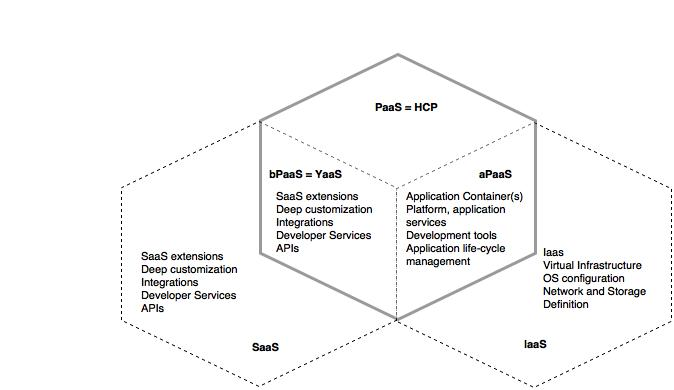
\includegraphics[width=0.8\textwidth]{figures/hybris-architecture-one}
\caption{\acrshort{YaaS} and \acrshort{HCP} \cite{Hirsch:2015aa}}
\label{fig:hybris_architecture/overview/yaas_overview}
\end{center}
\end{figure}
\\
\section{Vision}\label{section:hybris_architecture/vision}
The vision of \acrshort{YaaS} can be clarified with the following statement.
\begin{shaded}
"A cloud platform that allows everyone to easily develop, extend and sell services and applications." \\
\cite{Stubbe:2015aa}
\end{shaded}
The vision can be broadly categorized into following objectives.\\
\begin{enumerate}
\item \textbf{Cloud First}\\
The different parts of the application need to be scaled independently.
\item \textbf{Autonomy}\\
The development teams should be able to develop their modules independent of other teams and able to freely choose the technology that fits the job.
\item \textbf{Retain Speed}\\
The new features should be able to be released as fast as possible.
\item \textbf{Community}\\
It should be possible for the components to be shared across internal and external developers.
\end{enumerate}
The definition of microservices \ref{tab:context/microservices_architecture_style/keywords_extracted_from_various_definitions_of_microservice} as well as the characteristics of microservices [ref] signifies clearly that microservices architecture can be a good fit for \acrshort{YaaS} architecture.
\section{YaaS Architecture Principles}\label{section:hybris_architecture/YaaS_architecture_principles}
The Agile Manifesto \cite{Beck:2011aa} provides various principles to develop a software in a better way. It focus on fast response to the requirement changes with frequent continous delivery of software artifacts with close collaboration of customer and self-organizing teams.\\
Furthermore, the twelve factors from Heroku \cite{Wiggins:2012aa} provides methodology for minimizing time and cost to develop software applications as services. It emphasizes on scalability of applications, explicit declaration as well as isolation of dependencies among components, multiple continuous deployments from a single version controlled codebase with separate pipelines for build, release and run.\\
Finally, the microservices architecture provides techiques of developing an application as a collection of autonomous small sized services focused on single responsibility. [section \ref{section:context/microservices_architecture_style}] It focus on independent deployment capability of individual microservices and suggest to use lightweight mechanisms such as http for communication among services. Following the architecture offers various advantages not limited to individual independent scalability of each microservice, resilience by isolating failure in a component and technology heterogeneity among various development teams.\cite{Newman:2015aa}
 